\section{Ordering and Asynchrony}




\begin{figure}[t]
  \centering
  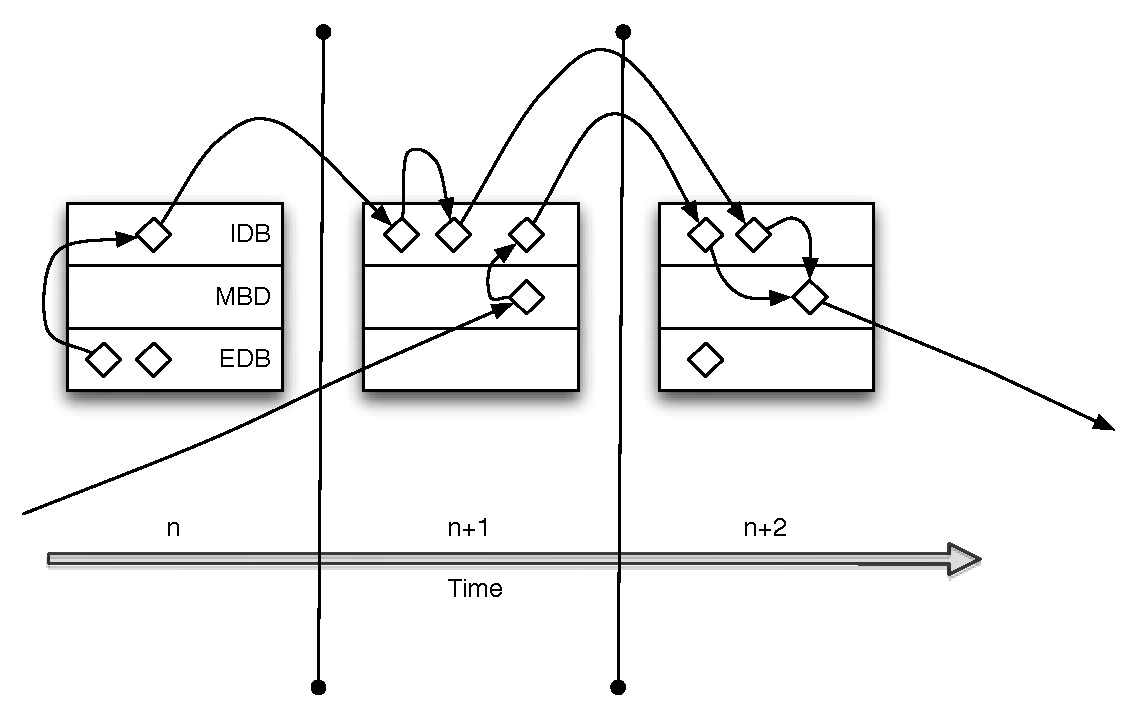
\includegraphics[width=1\linewidth]{edbidbmdb.pdf}
  \label{fig:edbidbmdb}
  \caption{Derivations across time in IDB and MDB relations.}
\vspace{-8pt}
\end{figure}


\section{Traces}

\paa{this section (its placement \emph{and} content) is somewhat problematic given the current structure
of the draft.  We've established the notion of finite prefixes of a (possibly infinite) EDB.  A trace is basically just
an interpretation (a set of ground atoms) -- by calling it a ``trace" we're connoting a post-hoc interpretation.
A trace that is just EDB is sufficient, given a program, to augment the trace with IDB and MDB atoms such that
the resulting trace is a model (by simply running a fixpoint computation).  For a program with no async rules, the EDB of input is sufficient to recreate the
program execution exactly -- that is to say, to reproduce the single minimal model of the program given the EDB.
It is \emph{not} sufficient to recreate the execution of a program with async rules: intuitively, we'd need to include in 
the trace the complete MDB, for every entry in it potentially corresponds to one of many possible minimal models.
perhaps we just want to show that there is a method (drop the async rules and run a fixpoint computation to generate
the IDB from MDB and EDB) to regenerate a "complete trace" (ie minimal model) from EDB $\cup$ MDB}

%Consider a non-empty EDB $E$, an empty MBD $M$ and IDB $I$ and a program $P$.  Evaluating $P$ against $E$ may derive facts in $M$ and $I$.

\begin{definition}
A \emph{trace} is any set of facts from the EDB, MDB or IDB of a Dedalus program evaluation.
\end{definition}

Any trace for a Dedalus instance $(P,E)$ is an interpretation of $(P,E)$.
%\wrm{lol, why do we need the notion of an incomplete trace?}

\begin{definition}
%
A \emph{complete trace} of an evaluation of a Dedalus instance is the union of
the given EDB with the derived IDB and MDB.
%
\end{definition}

\begin{lemma}
%
A complete trace of a Dedalus instance $(P,E)$ is its unique minimal model.
%
\end{lemma}

%\begin{lemma}
%%
%For any bound on $successor$, a complete trace of a Dedalus instance $(P,E)$ has a unique minimal model.
%%
%\end{lemma}

If we evaluate E given P, and P is stratifiable, the resulting set of ground atoms is a minimal model.
In our case, however, successor causes our EDB to be infinite, so the minimal model of any Dedalus program 
with temporal rules is potentially infinite.  \paa{but we'd like to show that a weaker property holds: that for any value $N$
in the \emph{successor} relation, the resulting program has a minimal model.}
\wrm{we either already showed this, or our theorems above are wrong.}


\begin{definition}
A \emph{minimal trace} is a subset of a complete trace that excludes any IDB ground atoms derived through an inductive
rule.
\end{definition}

A minimal trace of a Dedalus program $P$ is equivalent to the complete trace of which is is a subset -- the latter may be derived from the former by repeated
applications of inductive rules.  However, a given a Dedalus instance $(P, E)$ and a minimal trace T (where $E \subset T$), a fixpoint
computation will most likely \emph{not} yield a minimal model, because new tuples may be added to the MDB that represent a component 
of a different minimal model, and because these may affect the IDB.  The set of ground atoms $EDB \cup MDB_{old} \cup IDB_{new}$
\emph{may} may be a minimal model, iff $IDB_{new} = IDB_{old}$.  \paa{actually I am not sure if that is true}.  
$(EDB \cup MDB_{old} \cup IDB_{new} \cup IDB_{old})$ is certain to be a model, but is only minimal if $IDB_{new} \subset IDB_{old}$.

A minimal trace records the nondeterminism caused by the delay or reordering of async rules, and
is equivalent to the original program execution.  

\begin{definition}
A \emph{reduced trace} is a minimal trace with normalized time suffixes starting with 0 and increasing by 1 at each step.
\end{definition}

show a (trivial) procedure for reduction and make some claims about equivalences without entanglement.

\begin{definition}
A \emph{event trace} is a Dedalus EDB.
\end{definition}

An event trace and program P may be used to generate a new IDB and MDB.  The MDB is virtually certain to differ from that of another
execution, while the IDB may differ, depending on its dependency on the MDB.  The union of these three databases is of course a
minimal model, but probably not the same minimal model from another execution.  \paa{but can we say that it will often be true that if we project 
out the time attribute from every predicate, the minimal models will be the same? it won't always be true...}






\subsection{Queues}

%%Consider a trace of events to a 
Consider a predicate \emph{balance\_update} whose attributes are a string indicating the user, a floating point number
indicating the new balance and an integer indicating the order in which the updates were issued, according to some 
external clock or sequence.  

In this trace, all of the time suffixes are the same, e.g.

\begin{Dedalus}
balance\_update("bob", 100.00, 2355)@123;
balance\_update("bob", 75.00, 2358)@123;
balance\_update("alice", 0.00, 2377)@123;
balance\_update("bob", 10.00, 2455)@123;
\end{Dedalus}

Depending on the program that implements the balance update, several behaviors are possible.  We can see that in spite of their
coincidence in logical time, these events need to be processed in a data-dependent order, rather than as a set.  In-order tuple 
processing is difficult to express in Datalog generally, in part because the language has so notion of order of evaluation, except
the implicit ordering implied by stratification.

In the program below, we define a table \emph{m\_balance\_update} that we use as a queue to feed \emph{balance\_update}.  The queue must persist across
timesteps because it may take an unknown number of timesteps to drain it.  At each fixpoint, for each value of \textbf{A}, a single
tuple is projected into \emph{balance\_update} and atomically deleted from \emph{m\_balance\_update}, changing the value of the aggregate calculated at the
subsequent step:


\begin{Dedalus}

m\_balance\_update(A, B, C)@next \(\leftarrow\)
  m\_balance\_update(A, B, C),
  notin del\_m\_balance\_update(A, B, C);

omin(A, min<C>) \(\leftarrow\)
  m\_balance_update(A, _, C);

p(A, B, C)@next \(\leftarrow\)
  m\_balance\_update(A, B, C),
  omin(A, C);

del\_m\_balance\_update(A, B, C) \(\leftarrow\)
  m\_balance\_update(A, B, C),
  omin(A, C);
\end{Dedalus}

Under such a queueing discipline, deductive rules that are predicated on \emph{balance\_update} are constrained to consider only one tuple per fixpoint
per value of the variable \textbf{A}, thus implementing a per-user FIFO discipline.  To enforce a global FIFO ordering over \emph{balance\_update}, 
we may redefine \emph{omin} and any dependent rules to exclude the \textbf{A} atttribute.

A queue establishes a mapping between the local clock and the ordering domain of the input relation. By doing so, we are able to take
advantage of the natural ordering enforced by stratification over time, to enforce an ordering property over our input that is otherwise 
very difficult to express in a logic language.

\subsection{Lamport Clocks}

Implementing a Lamport Clock~\cite{timeclocks} is a special case of a queueing discipline as defined above.
Consider a predicate{m\_balance\_update} as defined above, but with an extra integer attribute that contains the logical transmission
time of the sender (via a message rule) of a given tuple.  For example, the sender's rule will look like: 

\paa{damn it!  we've sugared out N from the syntax!! now what?}

\begin{Dedalus}
m\_balance\_update(A, B, N)@async(N) \(\leftarrow\)
  send\_p(A, B);
\end{Dedalus}

Note that the time suffix is projected into the last attribute of \emph{m\_p}.  This establishes an \emph{entanglement} between
the sender's local clock and the program dataflow.  The queueing discipline that implements a
Lamport clock is then:

\begin{Dedalus}

m\_balance\_update(A, B, C)@next \(\leftarrow\)
  m\_balance\_update(A, B, C)@N,
  \(\lnot\) del\_m\_balance\_update(A, B, C)@N;

omin(A, min<C>)@N \(\leftarrow\)
  m\_balance\_update(A, B, C)@N;

lmin(min<C>)@N \(\leftarrow\)
  m\_balance\_update(_, _, C);

p(A, B, C)@N+1 :-
  m\_balance\_update(A, B, C)@N,
  omin(B)@N,
  lmax(L)@N,
  N > L;

del\_m\_balance\_update(A, B)@N :-
  m\_balance\_update(A, B)@N,
  omax(B)@N;
  
\end{Dedalus}



\subsection{Trace Entanglement}

